\chapter{Token distribution after tokenization}

\begin{figure}[htbp]
    \centering
    \captionsetup{font=small}
    \begin{subfigure}[b]{0.48\textwidth}
        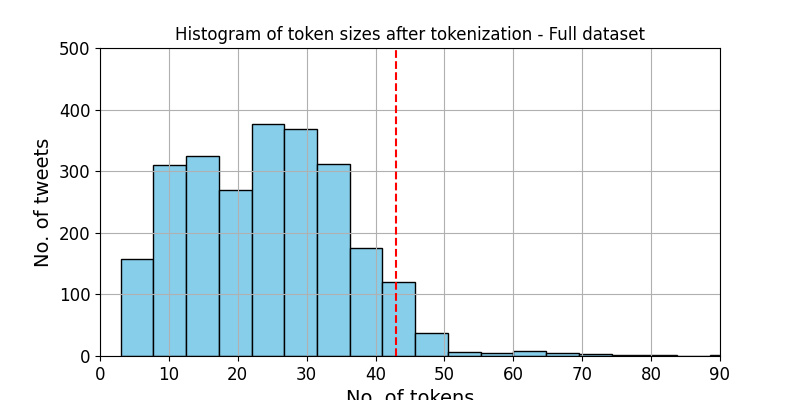
\includegraphics[width=\textwidth]{figures/token_pp_hist_albert-base-v2.png}
        \caption{Albert base}
        \label{fig: token_pp_hist_albert}
    \end{subfigure}
    \hfill
    \begin{subfigure}[b]{0.48\textwidth}
        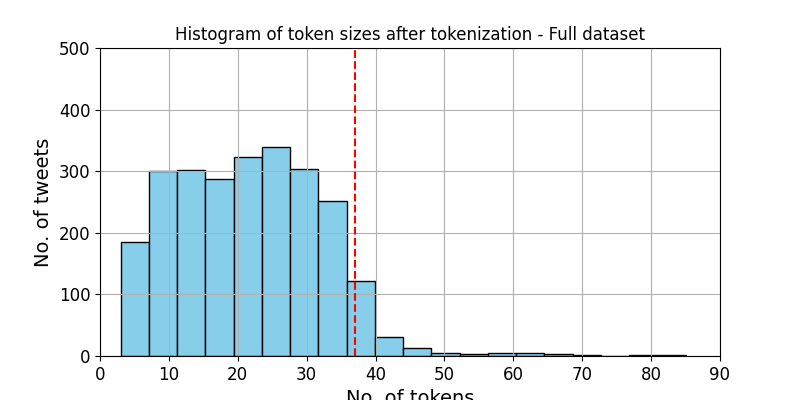
\includegraphics[width=\textwidth]{figures/token_pp_hist_distilbert-base-uncased.png}
        \caption{DistilBERT base uncase}
        \label{fig: token_pp_hist_distilbert}
    \end{subfigure}
    \begin{subfigure}[b]{0.48\textwidth}
        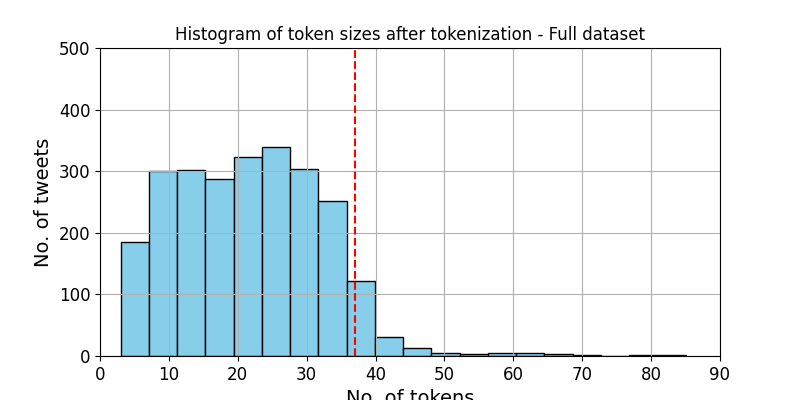
\includegraphics[width=\textwidth]{figures/token_pp_hist_google-mobilebert-uncased.png}
        \caption{MobileBERT uncased}
        \label{fig: token_pp_hist_mobile}
    \end{subfigure}
    \hfill
    \begin{subfigure}[b]{0.48\textwidth}
        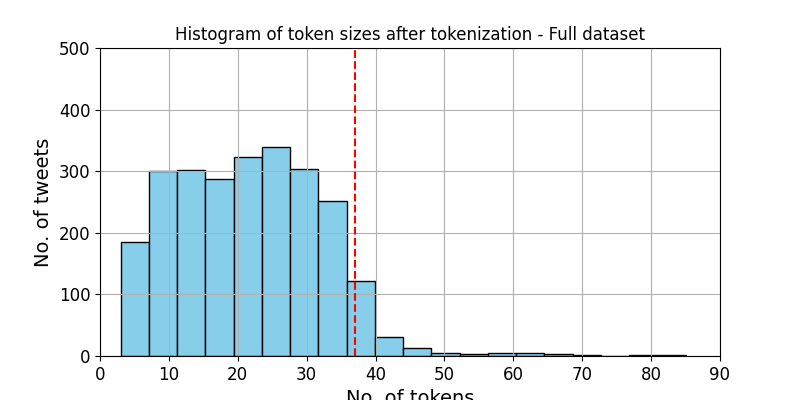
\includegraphics[width=\textwidth]{figures/token_pp_hist_prajjwal1-bert-tiny.png}
        \caption{BERT tiny}
        \label{fig: token_pp_hist}
    \end{subfigure}
    \caption{The token count distribution for the full dataset of 3,449 tweets before and after tokenization with the red dashed line indicating 95\% coverage of tweets. BertTokenizer is used here.}
    \label{fig: bef_aft_token}
    \begin{subfigure}[b]{0.48\textwidth}
        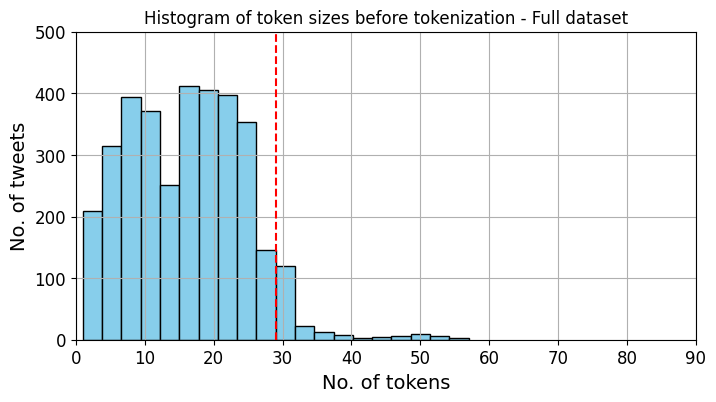
\includegraphics[width=\textwidth]{figures/token_hist.png}
        \caption{Before tokenization}
        \label{fig: token_hist}
    \end{subfigure}
    \hfill
    \begin{subfigure}[b]{0.48\textwidth}
        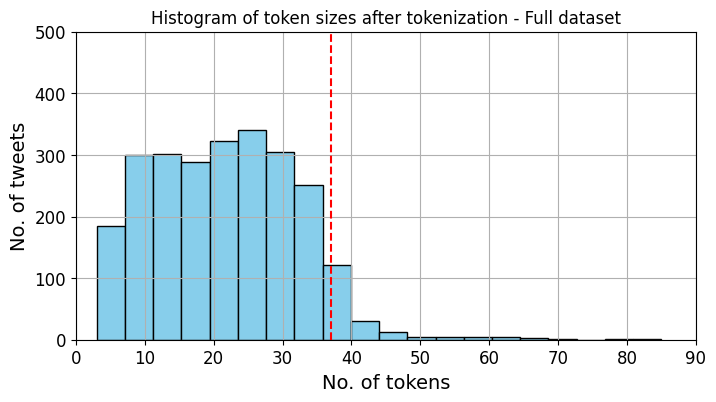
\includegraphics[width=\textwidth]{figures/token_pp_hist.png}
        \caption{After tokenization}
        \label{fig: token_pp_hist}
    \end{subfigure}
    \caption{The token count distribution for the full dataset of 3,449 tweets before and after tokenization with the red dashed line indicating 95\% coverage of tweets. BertTokenizer is used here.}
    \label{fig: bef_aft_token}
\end{figure}

